% ----------------------------------------------------
% -------- BAYSIS - Selected as Jam Effector ---------
% ----------------------------------------------------
\subsection{Congestion - Accidents categorizes as Jam Effector}
\label{analysis_processing_correlation_baysis_effector}
The correlation matrix table for the congestion - accident dataset, which are classified as \textit{Jam Effector} (see \cref{table:appendix_correlation_matrix_matched_cramers}) is visual presented in \cref{img:correlation_matrix_selected_effector_cramers} showing the the correlation of each variable combination. When visual analyzing \cref{img:correlation_matrix_matched_cramers} and checking the guidelines for a strong correlation in reference to the applied coefficient (identifiable with \cref{table:appendix_coefficient_matrix_matched}) we get a list of strongly correlated variable combinations (see \cref{tbl:correlation_list_baysis_effector}). Since the focus of the thesis are the correlations between accidents and jams, these are only collected from the bottom-left rectangle of the matrix, where the congestion and accidents variables intersect. Correlations of the kind congestion - congestion or accident - accident are not considered.
\begin{table}[h!]
	\centering
	\begin{tabular}{c|l}  
		Category & Strong \\
		\\[-1em]
		\hline
		\\[-1em]
		Strasse & TMax, TAvg, SMax, SAvg, Cov, TLHGV \\ 
 		Kat & TMax, TAvg, SAvg \\ % + SMax % -> Strasse
 		%Typ & \\ % -> Strasse
 		%Betei & \\
 		UArt1 & SAvg \\ % -> Strasse
 		%UArt2 & \\ % -> Strasse
 		%AUrs1 & \\ % -> Strasse
 		%AUrs2 & \\
 		AufHi & TMax, TAvg \\
 		%Alkoh & \\
 		%Char1 & \\ % -> Strasse
 		%Char2 & \\ % -> Strasse
 		%Lich1 & \\ % -> Strasse
 		%Lich2 & \\ % -> Strasse
 		%Zust1 & \\ % -> Strasse
 		%Zust2 & \\ % -> Strasse
 		%Fstf & \\ % -> Strasse
 		WoTag & TAvg, SMax, Cov, TLHGV \\ % -> Strasse
 		%FeiTag & \\
 		Month & TMax, TAvg, SMax, SAvg, Cov, TLHGV \\ % -> Strasse
	\end{tabular}
    \caption{List of incident variables and their strong correlated congestion variable from the congestion-accident matched data which are classified as \textit{Jam Effector}}
	\label{tbl:correlation_list_baysis_effector}
\end{table}
Next we need to verify that the correlation is significant and what the correlation predicates. Therefore each correlation will be evaluated with the Post Hoc test, defined in \cref{correlation_posthoc}. \secintroend{baysis}{effector}
\begin{figure}[!ht]
	\centering
	\makebox[\textwidth][c]{%
		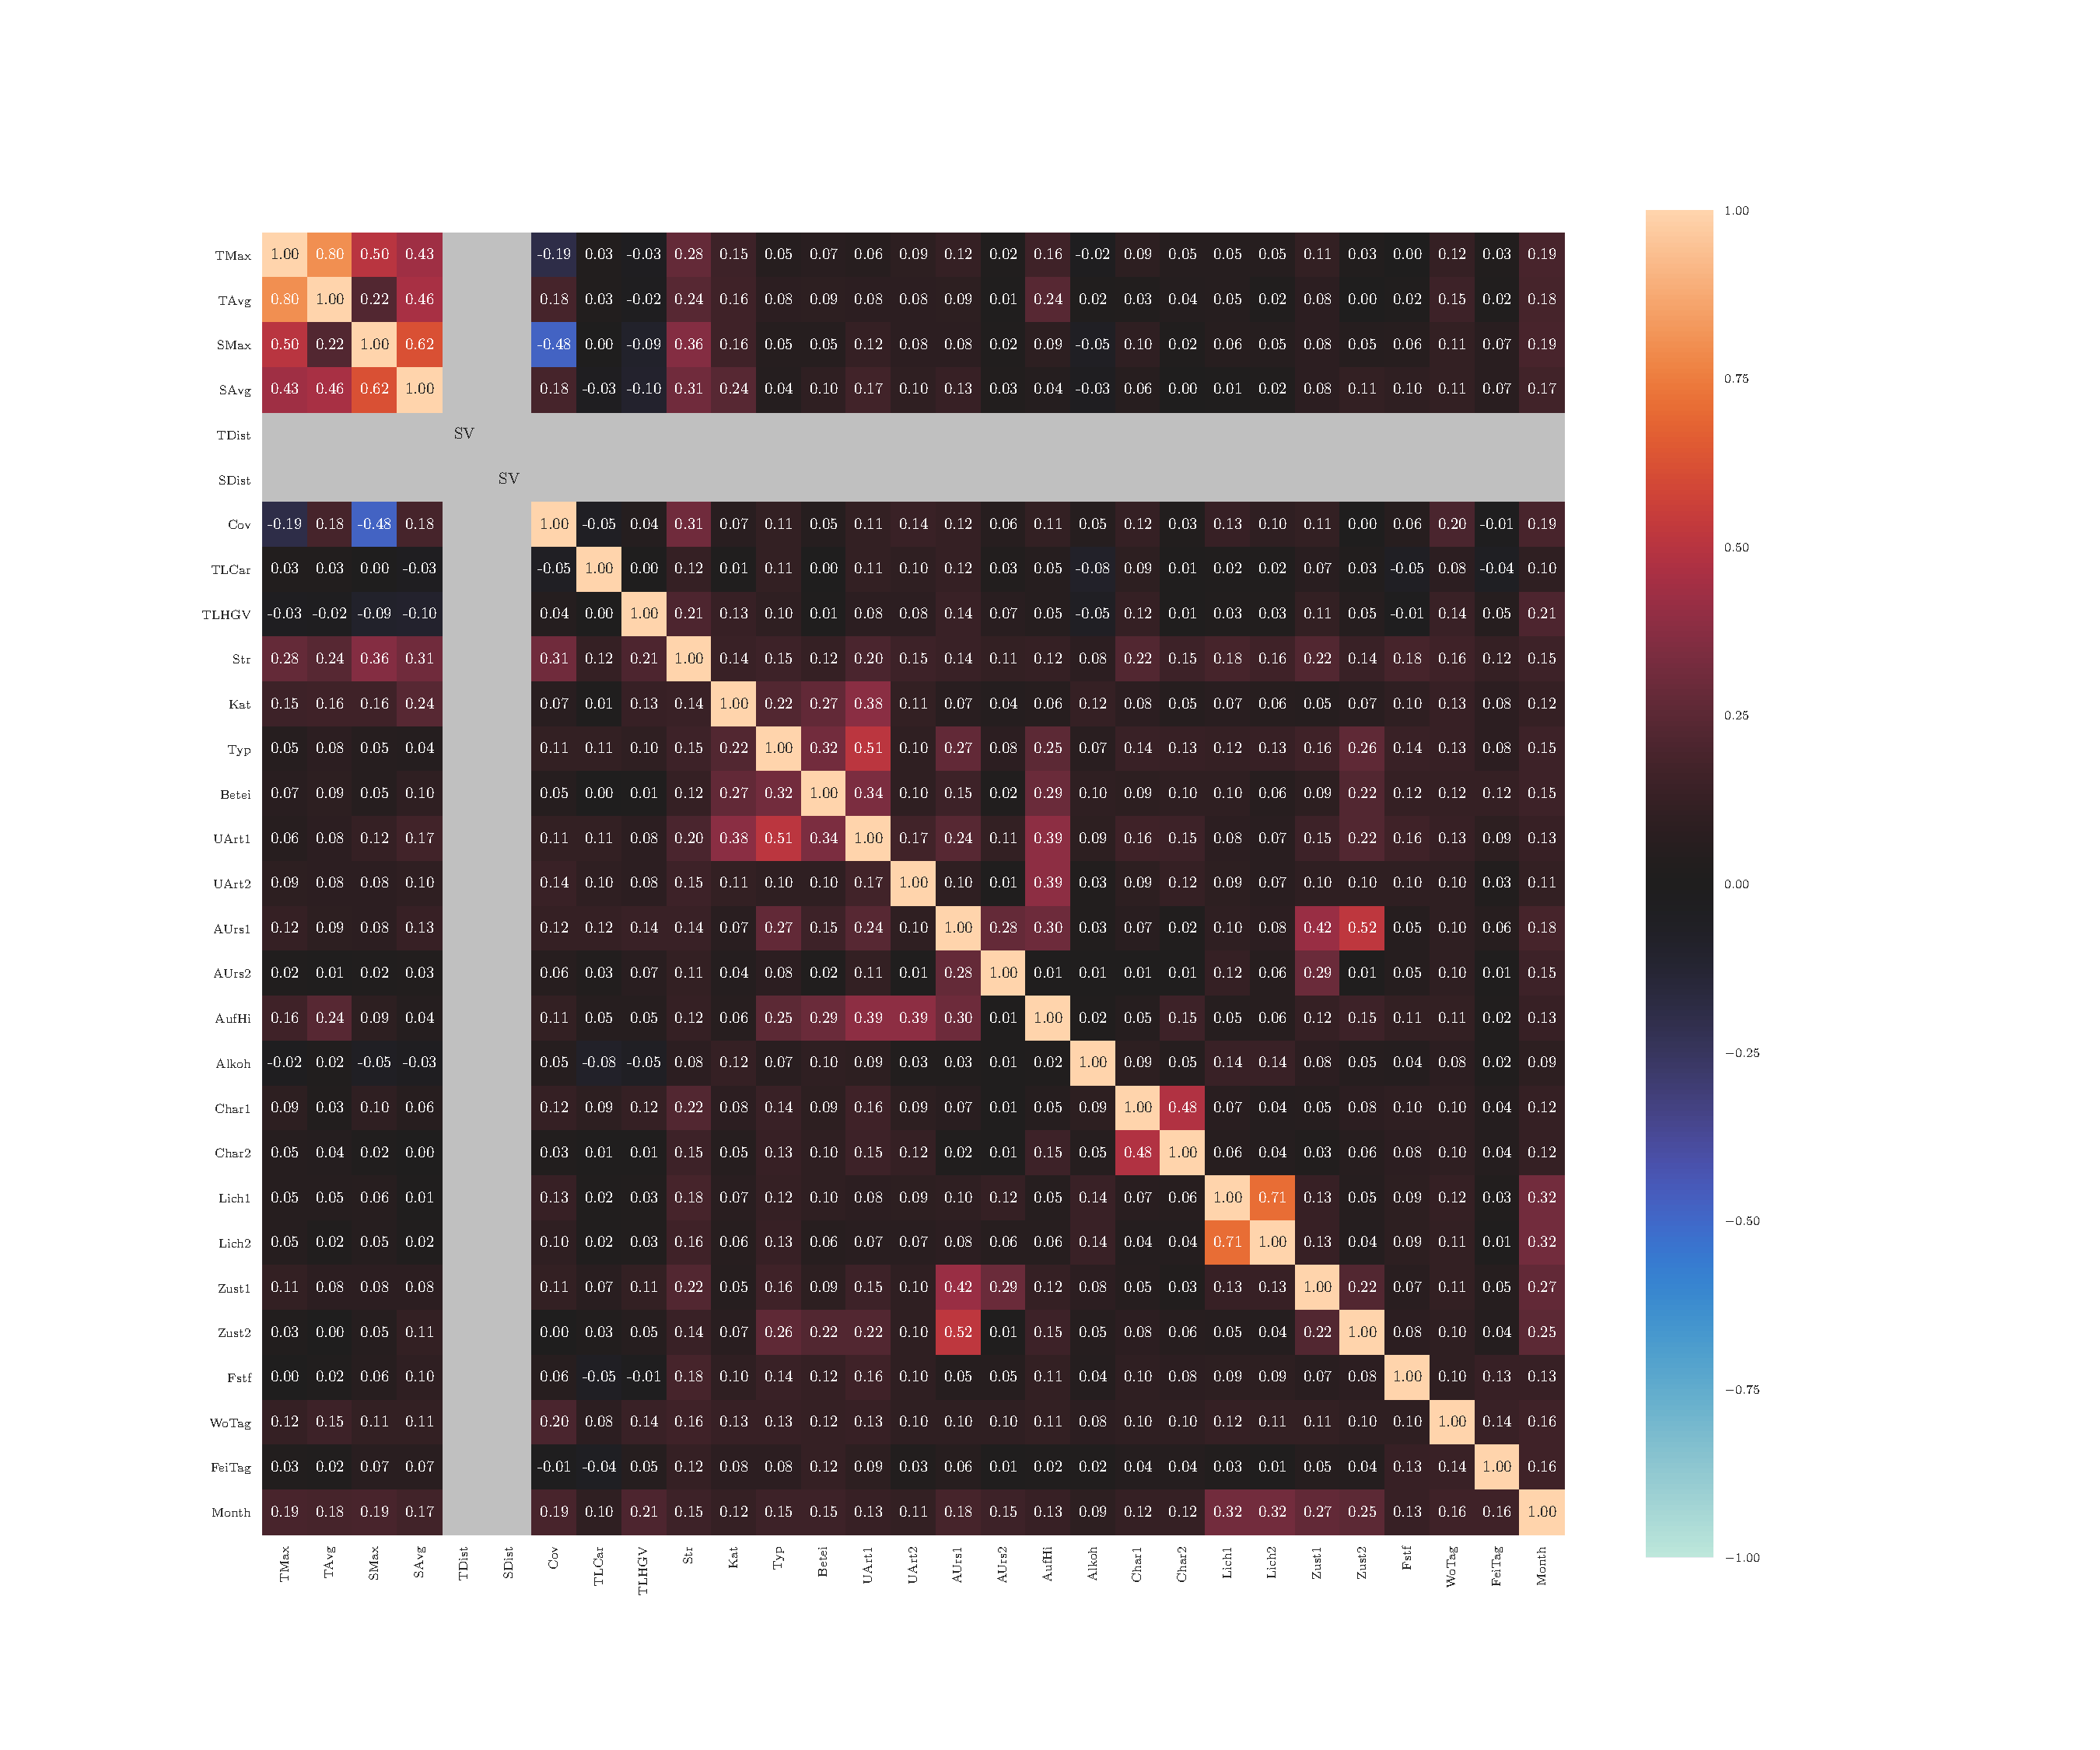
\includegraphics[width=1.4\textwidth, trim=0cm 2.5cm 6cm 3cm]{CorrAnalysis/data/BAYSIS/03_selected_02_duringJam/plots/baysis_selected_corr_cramers}%
	}
	\caption{Correlation matrix for congestion-accident matched data classified as \textit{Jam Effector} and calculated with $V$, $\eta$, $\tau$, $r_{pq}$, $r$}
	\label{img:correlation_matrix_selected_effector_cramers}
\end{figure}

% --------------------------
% -------- Street ---------
% --------------------------
\centerheading{Street}
\label{ana:baysis_effector_Str}
\varintrosimplewithsam{Str}
\varintronosigmul{Str}{\textit{Strasse} - \textit{SAvg} and \textit{Strasse} - \textit{TLHGV}}

% #################################################
\groupintrosig{Street}{TMax}{0.0104}{baysis}{effector}
\begin{table}[ht!]
	\tiny
	\centering
	\begin{tabular}{rrrrrrrrrrrrrr}
		\toprule
		     & A3 & A6 & A9 & A70 & A99 & A93 & A94 & A7 & A73 & A96 & A995 & A92 & A95 \\ 
		\midrule
		% A6   & 1.00 &  &  &  &  &  &  &  &  &  &  &  &  \\ 
		% A9   & 1.00 & 1.00 &  &  &  &  &  &  &  &  &  &  &  \\ 
		% A70  & 1.00 & 1.00 & 1.00 &  &  &  &  &  &  &  &  &  &  \\ 
		% A99  & 0.85 & 1.00 & 1.00 & 1.00 &  &  &  &  &  &  &  &  &  \\ 
		% A93  & 1.00 & 1.00 & 1.00 & 1.00 & 1.00 &  &  &  &  &  &  &  &  \\ 
		A94  & \red{0.01} & 1.00 & 0.06 & 1.00 & 0.28 & 1.00 &  &  &  &  &  &  &  \\ 
		% A7   & .00 & 1.00 & 1.00 & 1.00 & 1.00 & 1.00 & 1.00 &  &  &  &  &  &  \\ 
		A73  & \red{0.00} & 1.00 & \red{0.00} & 1.00 & 0.23 & 1.00 & 1.00 & 1.00 &  &  &  &  &  \\ 
		A96  & \red{0.00} & 1.00 & 0.35 & 1.00 & 1.00 & 1.00 & 1.00 & 1.00 & 1.00 &  &  &  &  \\ 
		% A995 & 1.00 & 1.00 & 1.00 & 1.00 & 1.00 & 1.00 & 1.00 & 1.00 & 1.00 & 1.00 &  &  &  \\ 
		A92  & \red{0.01} & 1.00 & 0.24 & 1.00 & 1.00 & 1.00 & 1.00 & 1.00 & 1.00 & 1.00 & 1.00 &  &  \\ 
		% A95  & 1.00 & 1.00 & 1.00 & 1.00 & 1.00 & 1.00 & 1.00 & 1.00 & 1.00 & 1.00 & 1.00 & 1.00 &  \\ 
		% A980 & 1.00 & 1.00 & 1.00 & 1.00 & 1.00 & 1.00 & 1.00 & 1.00 & 1.00 & 1.00 & 1.00 & 1.00 &  \\ 
		\bottomrule
	  \end{tabular}
    \caption{Pairwise Wilcoxon $T$-test for \textit{Street} and \textit{Maximal Temporal Extent} (Jam Effector)}
    \label{tbl:wilcoxon_baysis_effector_Street_TMax}
\end{table}
The table shows that the roads A73, A94, A95 and A96 differ from the A3. The A73 also differs from the A9, but there is no distinctive general trend.
% #### START: Table and Plot
\begin{figure}[ht!]
	\centering
	\begin{minipage}{0.5\textwidth}
		\tiny
		\setlength{\tabcolsep}{4pt}
		\centering
		\begin{tabular}{c|c|c|c|c|c|c|c}
			\toprule
			Group & $n$ & $\bar{x}$ & $\sigma$ & $\tilde{x}$ & $min$ & $max$ & $\Delta$ \\
			\midrule
			A3   & 265 & 297.62 & 219.09 & 243.0 & 18 & 1257 & 1239 \\ 
			A6   & 37  & 236.59 & 183.03 & 207.0 & 18 & 705  & 687  \\ 
			A9   & 192 & 243.45 & 178.97 & 201.0 & 15 & 1194 & 1179 \\ 
			A99  & 63  & 212.57 & 140.78 & 195.0 & 21 & 681  & 660  \\ 
			A93  & 12  & 212.00 & 187.74 & 130.5 & 39 & 588  & 549  \\ 
			A94  & 14  & 109.71 & 56.07  & 97.5  & 42 & 249  & 207  \\ 
			A7   & 35  & 254.66 & 306.21 & 168.0 & 42 & 1341 & 1299 \\ 
			A73  & 52  & 157.21 & 179.42 & 130.5 & 18 & 1323 & 1305 \\ 
			A96  & 41  & 155.85 & 84.33  & 144.0 & 30 & 381  & 351  \\ 
			A92  & 21  & 134.71 & 82.25  & 138.0 & 18 & 354  & 336  \\ 
			\bottomrule
			% \bar{x} - sum = 2014.37, mean = 201,43
			% \sigma - sum = 1617.89, mean = 161.78
			% \tilde{x}
		\end{tabular}
		\subcaption[second caption.]{Table of all descriptives}\label{tbl:descriptives_baysis_effector_Street_TMax}
	\end{minipage}%
	\begin{minipage}{0.55\textwidth}
		\pgfplotstableread[col sep=comma]{
			road, count, mean, median, sd, min, max, delta
			A3   , 265 , 297.62 , 219.09 , 243.0 , 18 , 1257 , 1239
			A6   , 37  , 236.59 , 183.03 , 207.0 , 18 , 705  , 687 
			A9   , 192 , 243.45 , 178.97 , 201.0 , 15 , 1194 , 1179
			A99  , 63  , 212.57 , 140.78 , 195.0 , 21 , 681  , 660 
			A93  , 12  , 212.00 , 187.74 , 130.5 , 39 , 588  , 549 
			A94  , 14  , 109.71 , 56.07  , 97.5  , 42 , 249  , 207 
			A7   , 35  , 254.66 , 306.21 , 168.0 , 42 , 1341 , 1299
			A73  , 52  , 157.21 , 179.42 , 130.5 , 18 , 1323 , 1305
			A96  , 41  , 155.85 , 84.33  , 144.0 , 30 , 381  , 351 
			A92  , 21  , 134.71 , 82.25  , 138.0 , 18 , 354  , 336 
		}\data
        \pgfplotstablesort[sort key=mean, sort cmp=float >]{\datasorted}{\data}
        \tiny
        \centering
        \descplotfigwithavg{\datasorted}{201}{161}{10}{4.7}
		\subcaption[second caption.]{Plot of descriptives $\bar{x}$, $\sigma$ and $\tilde{x}$}\label{fig:descriptives_baysis_effector_Street_TMax}
	\end{minipage}%
	\caption{Group descriptives of \textit{Street} and \textit{Maximal Temporal Extent} (Jam Effector)}
	%\vspace{-8mm}
\end{figure}
% #### END: Table and Plot
The descriptives from \cref{tbl:descriptives_baysis_effector_Street_TMax} show that the A94, A73 and A96 (the A95 is uncertain) have a mean maximal temporal distance of 140\,min. Compared to the $\bar{x}$ of the A3 of 311\,min it can be interpreted that accidents on the A3 is associated with twice as long jams than the other groups. For the A9 can be interpreted that it's accidents are associated with 40\,\% longer jams, than the A73.

% ####################################################
\groupintrosig{Street}{TAvg}{0.0003}{baysis}{effector}
\begin{table}[ht!]
	\tiny
	\centering
	\begin{tabular}{rrrrrrrrrrrrrr}
		\toprule
			 & A3 & A6 & A9 & A70 & A99 & A93 & A94 & A7 & A73 & A96 & A995 & A92 & A95 \\ 
		\midrule
		% A6   & 1.00 &  &  &  &  &  &  &  &  &  &  &  &  \\ 
		% A9   & 1.00 & 1.00 &  &  &  &  &  &  &  &  &  &  &  \\ 
		% A70  & 1.00 & 1.00 & 1.00 &  &  &  &  &  &  &  &  &  &  \\ 
		A99  & \red{0.02} & 1.00 & 1.00 & 1.00 &  &  &  &  &  &  &  &  &  \\ 
		% A93  & 1.00 & 1.00 & 1.00 & 1.00 & 1.00 &  &  &  &  &  &  &  &  \\ 
		% A94  & 0.11 & 1.00 & 0.53 & 1.00 & 1.00 & 1.00 &  &  &  &  &  &  &  \\ 
		% A7   & 1.00 & 1.00 & 1.00 & 1.00 & 1.00 & 1.00 & 0.61 &  &  &  &  &  &  \\ 
		A73  & \red{0.00} & 1.00 & 0.00 & 1.00 & 1.00 & 1.00 & 1.00 & \red{0.02} &  &  &  &  &  \\ 
		% A96  & 1.00 & 1.00 & 1.00 & 1.00 & 1.00 & 1.00 & 1.00 & 1.00 & 0.87 &  &  &  &  \\ 
		% A995 & 1.00 & 1.00 & 1.00 & 1.00 & 1.00 & 1.00 & 1.00 & 1.00 & 1.00 & 1.00 &  &  &  \\ 
		% A92  & 1.00 & 1.00 & 1.00 & 1.00 & 1.00 & 1.00 & 1.00 & 1.00 & 1.00 & 1.00 & 1.00 &  &  \\ 
		% A95  & 1.00 & 1.00 & 1.00 & 1.00 & 1.00 & 1.00 & 1.00 & 1.00 & 1.00 & 1.00 & 1.00 & 1.00 &  \\ 
		% A980 & 1.00 & 1.00 & 1.00 & 1.00 & 1.00 & 1.00 & 1.00 & 1.00 & 1.00 & 1.00 & 1.00 & 1.00 & 1.00 \\ 
		\bottomrule
	  \end{tabular}
    \caption{Pairwise Wilcoxon $T$-test for \textit{Strasse} and \textit{Average Temporal Extent} (Jam Effector)}
    \label{tbl:wilcoxon_baysis_effector_Street_TAvg}
\end{table}
The table shows that the roads A99 and A73 differ from the A3. The A73 also differs from A7.
% #### START: Table and Plot
\begin{figure}[ht!]
	\centering
	\begin{minipage}{0.5\textwidth}
		\tiny
		\centering
		\begin{tabular}{c|c|c|c|c|c|c|c}
			\toprule
			Group & $n$ & $\bar{x}$ & $\sigma$ & $\tilde{x}$ & $min$ & $max$ & $\Delta$ \\
			\midrule
			A3   & 265 & 104.05 & 87.02  & 84 & 7  & 703  & 696  \\ 
			A6   & 37  & 82.43  & 74.19  & 70 & 3  & 301  & 298  \\ 
			A9   & 192 & 91.31  & 74.64  & 75 & 5  & 575  & 570  \\  
			A99  & 63  & 65.73  & 47.32  & 52 & 4  & 295  & 291  \\ 
			A93  & 12  & 104.83 & 112.03 & 55 & 7  & 343  & 336  \\ 
			A94  & 14  & 45.93  & 25.54  & 43 & 14 & 102  & 88   \\ 
			A7   & 35  & 143.74 & 255.78 & 76 & 15 & 1326 & 1311 \\ 
			A73  & 52  & 47.63  & 29.09  & 44 & 6  & 154  & 148  \\ 
			A96  & 41  & 74.39  & 54.53  & 70 & 6  & 247  & 241  \\ 
			A92  & 21  & 64.52  & 48.86  & 56 & 8  & 235  & 227  \\ 
			\bottomrule
			% \bar{x} - sum = 824.56, mean = 82.45
			% \sigma - sum = 809, mean = 80.9
			% \tilde{x}
		\end{tabular}
		\subcaption[second caption.]{Table of all descriptives}\label{tbl:descriptives_baysis_effector_Street_TAvg}
	\end{minipage}%
	\begin{minipage}{0.55\textwidth}
		\pgfplotstableread[col sep=comma,header=false]{
			A3   , 265 , 104.05 , 87.02  , 84 , 7  , 703  , 696 
			A6   , 37  , 82.43  , 74.19  , 70 , 3  , 301  , 298 
			A9   , 192 , 91.31  , 74.64  , 75 , 5  , 575  , 570  
			A99  , 63  , 65.73  , 47.32  , 52 , 4  , 295  , 291 
			A93  , 12  , 104.83 , 112.03 , 55 , 7  , 343  , 336 
			A94  , 14  , 45.93  , 25.54  , 43 , 14 , 102  , 88  
			A7   , 35  , 143.74 , 255.78 , 76 , 15 , 1326 , 1311
			A73  , 52  , 47.63  , 29.09  , 44 , 6  , 154  , 148 
			A96  , 41  , 74.39  , 54.53  , 70 , 6  , 247  , 241 
			A92  , 21  , 64.52  , 48.86  , 56 , 8  , 235  , 227 
		}\data
		\tiny
		\centering
		\begin{tikzpicture}
			\begin{axis}[
				% Gitterlinien für y-Ticks
				width=\textwidth,
				height=4.7cm,
				xmajorgrids=true,
				ymajorgrids=true,
				xtick=data,
				xmin=0,xmax=9,
				xticklabels from table={\data}{[index]0},
				% zusätzliche Beschriftung an y-Achse
				every extra y tick/.style={
					tick0/.initial=blue,
					tick1/.initial=red,
					yticklabel style={
						color=\pgfkeysvalueof{/pgfplots/tick\ticknum}
					},
				},
				extra y ticks={82,81},
			]
			\addplot table [absolute series=2] {\data};
			\addplot table [absolute series=3] {\data};
			\addplot table [absolute series=4] {\data};
			\legend{
				$\bar{x}$,$\sigma$,$\tilde{x}$}
			\end{axis}
		 \end{tikzpicture}\vfill
		\subcaption[second caption.]{Plot of descriptives $\bar{x}$, $\sigma$ and $\tilde{x}$}\label{fig:descriptives_baysis_effector_Street_TAvg}
	\end{minipage}%
	\caption{Group descriptives of \textit{Street} and \textit{Average Temporal Extent} (Jam Effector)}
	%\vspace{-8mm}
\end{figure}
% #### END: Table and Plot
The descriptives in \cref{tbl:descriptives_baysis_effector_Street_TAvg,fig:descriptives_baysis_effector_Street_TAvg} show that the mean $\bar{x}$ of the groups A99 and A73 is 56\,min, which is nearly 50\,\% lower than the $\bar{x}$ of A3. The $\bar{x}$ of A73 is also just $\frac{1}{3}$ compared to the A94. It can be interpreted that accidents on the A3 and A7 are associated with significantly longer jams than on other roads.
\begin{figure}[ht!]
	\pgfplotstableread[col sep=comma]{
		Road, meanTMax, meanTAvg
		A3  , 297.62  , 104.05
		A6  , 236.59  , 82.43 
		A9  , 243.45  , 91.31 
		A99 , 212.57  , 65.73 
		A93 , 212.00  , 104.83
		A94 , 109.71  , 45.93 
		A7  , 254.66  , 143.74
		A73 , 157.21  , 47.63 
		A96 , 155.85  , 74.39 
		A92 , 134.71  , 64.52   
	}\data 
	\tiny
	\centering
	\barplotdoubleanalysis{\data}{meanTMax}{meanTAvg}{$\bar{x}_{TMax}$}{$\bar{x}_{TAvg}$}
	\caption{Comparison of descriptives $\bar{x}_{SMax}$ and $\bar{x}_{SAvg}$ (\textit{Street} by \textit{TMax/TAvg})}
	\label{fig:baysis_effector_meancomparison_Str_spatial}
	%\vspace{-8mm}
\end{figure}
When comparison the mean values of the maximal and average (temporal) extend it becomes clear that the average is significantly lower than the maximum, which is to be expected. It shows, that the differences between the groups are similar in both the maximal and average extend.

% ####################################################
\groupintrosig{Street}{SMax}{0.0025}{baysis}{effector}
\begin{table}[ht!]
	\tiny
	\centering
	\begin{tabular}{rrrrrrrrrrrrrr}
		\toprule
			 & A3 & A6 & A9 & A70 & A99 & A93 & A94 & A7 & A73 & A96 & A995 & A92 & A95 \\ 
		\midrule
		% A6   & 1.00 &  &  &  &  &  &  &  &  &  &  &  &  \\ 
		A9   & \red{0.00} & 1.00 &  &  &  &  &  &  &  &  &  &  &  \\ 
		% A70  & 1.00 & 1.00 & 1.00 &  &  &  &  &  &  &  &  &  &  \\ 
		% A99  & 1.00 & 1.00 & 1.00 & 1.00 &  &  &  &  &  &  &  &  &  \\ 
		A93  & 0.07 & 0.13 & 1.00 & 1.00 & 1.00 &  &  &  &  &  &  &  &  \\ 
		A94  & \red{0.01} & \red{0.03} & 0.41 & 1.00 & 0.24 & 1.00 &  &  &  &  &  &  &  \\ 
		A7   & 0.08 & 0.65 & 1.00 & 1.00 & 1.00 & 1.00 & 1.00 &  &  &  &  &  &  \\ 
		A73  & \red{0.00} & \red{0.00} & \red{0.00} & 1.00 & \red{0.00} & 1.00 & 1.00 & 0.95 &  &  &  &  &  \\ 
		A96  & 0.13 & 1.00 & 1.00 & 1.00 & 1.00 & 1.00 & 1.00 & 1.00 & 0.18 &  &  &  &  \\ 
		% A995 & 1.00 & 1.00 & 1.00 & 1.00 & 1.00 & 1.00 & 1.00 & 1.00 & 1.00 & 1.00 &  &  &  \\ 
		A92  & \red{0.00} & \red{0.00} & \red{0.04} & 1.00 & \red{0.04} & 1.00 & 1.00 & 1.00 & 1.00 & 1.00 & 1.00 &  &  \\ 
		% A95  & 1.00 & 1.00 & 1.00 & 1.00 & 1.00 & 1.00 & 1.00 & 1.00 & 1.00 & 1.00 & 1.00 & 1.00 &  \\ 
		% A980 & 1.00 & 1.00 & 1.00 & 1.00 & 1.00 & 1.00 & 1.00 & 1.00 & 1.00 & 1.00 & 1.00 & 1.00 & 1.00 \\ 
		\bottomrule
	  \end{tabular}
    \caption{Pairwise Wilcoxon $T$-test for \textit{Street} and \textit{Maximal Spatial Extent} (Jam Effector)}
    \label{tbl:wilcoxon_baysis_effector_Street_SMax}
\end{table}
The table shows that the roads of A9, A73, and A92 differ significantly from A3. The roads A94, A73 and A92 also differ significantly from A6. A73 and A92 also differ significantly from A9 and A99, but there is no distinctive trend.
% #### START: Table and Plot
\pgfplotstableread[col sep=comma,header=false]{
	A3   , 265 , 17755.15 , 11139.22 , 14811.0 , 1566 , 46328 , 44762 
	A6   , 37  , 16711.43 , 9518.81  , 14449.0 , 2655 , 40033 , 37378 
	A9   , 192 , 13271.42 , 8473.71  , 11654.5 , 1315 , 49765 , 48450 
	A99  , 63  , 17558.70 , 12223.42 , 14698.0 , 2351 , 48278 , 45927 
	A93  , 12  , 8158.42  , 4473.23  , 7461.5  , 2896 , 16922 , 14026 
	A94  , 14  , 7277.64  , 4218.45  , 6947.0  , 1206 , 15550 , 14344 
	A7   , 35  , 11825.00 , 8885.99  , 9506.0  , 3041 , 43244 , 40203 
	A73  , 52  , 7964.98  , 5995.59  , 6559.5  , 1036 , 33764 , 32728 
	A96  , 41  , 11825.98 , 6911.19  , 9676.0  , 2006 , 27965 , 25959 
	A92  , 21  , 7255.76  , 3637.71  , 7364.0  , 1176 , 13522 , 12346 
}\data
\pgfplotstablecreatecol[
  create col/expr={\thisrow{1} + \thisrow{2} + \thisrow{3} + \thisrow{4}}
]{sum}{\data}
\begin{figure}[ht!]
	\centering
	\begin{minipage}{0.5\textwidth}
		\tiny
		\setlength{\tabcolsep}{4pt}
		\centering
		\begin{tabular}{c|c|c|c|c|c|c|c}
			\toprule
			Group & $n$ & $\bar{x}$ & $\sigma$ & $\tilde{x}$ & $min$ & $max$ & $\Delta$ \\
			\midrule
			A3   & 265 & 17755.15 & 11139.22 & 14811.0 & 1566 & 46328 & 44762 \\ 
			A6   & 37  & 16711.43 & 9518.81  & 14449.0 & 2655 & 40033 & 37378 \\ 
			A9   & 192 & 13271.42 & 8473.71  & 11654.5 & 1315 & 49765 & 48450 \\ 
			A99  & 63  & 17558.70 & 12223.42 & 14698.0 & 2351 & 48278 & 45927 \\ 
			A93  & 12  & 8158.42  & 4473.23  & 7461.5  & 2896 & 16922 & 14026 \\ 
			A94  & 14  & 7277.64  & 4218.45  & 6947.0  & 1206 & 15550 & 14344 \\ 
			A7   & 35  & 11825.00 & 8885.99  & 9506.0  & 3041 & 43244 & 40203 \\ 
			A73  & 52  & 7964.98  & 5995.59  & 6559.5  & 1036 & 33764 & 32728 \\ 
			A96  & 41  & 11825.98 & 6911.19  & 9676.0  & 2006 & 27965 & 25959 \\ 
			A92  & 21  & 7255.76  & 3637.71  & 7364.0  & 1176 & 13522 & 12346 \\ 
			\bottomrule
			% \bar{x} - sum = 119604.48, mean = 11960.44
			% \sigma - sum = 75477.32, mean = 7547.73
			% \tilde{x}
		\end{tabular}
		\subcaption[second caption.]{Table of all descriptives}\label{tbl:descriptives_baysis_effector_Street_SMax}
	\end{minipage}%
	\begin{minipage}{0.55\textwidth}
		\tiny
		\centering
		\begin{tikzpicture}
			\begin{axis}[
				% Gitterlinien für y-Ticks
				width=\textwidth,
				height=4.7cm,
				xmajorgrids=true,
				ymajorgrids=true,
				xtick=data,
				xmin=0,xmax=9,
				xticklabels from table={\data}{[index]0},
				% zusätzliche Beschriftung an y-Achse
				every extra y tick/.style={
					tick0/.initial=blue,
					tick1/.initial=red,
					yticklabel style={
						color=\pgfkeysvalueof{/pgfplots/tick\ticknum}
					},
				},
				extra y ticks={11960,7547},
				extra y tick labels={1.19,0.75}
			]
			\addplot table [absolute series=2] {\data};
			\addplot table [absolute series=3] {\data};
			\addplot table [absolute series=4] {\data};
			\legend{
				$\bar{x}$,$\sigma$,$\tilde{x}$}
			\end{axis}
		 \end{tikzpicture}\vfill
		\subcaption[second caption.]{Plot of descriptives $\bar{x}$, $\sigma$ and $\tilde{x}$}\label{fig:descriptives_baysis_effector_Street_SMax}
	\end{minipage}%
	\caption{Group descriptives of \textit{Street} and \textit{Maximal Spatial Extent} (Jam Effector)}
	%\vspace{-8mm}
\end{figure}
% #### END: Table and Plot
The descriptives in \cref{tbl:descriptives_baysis_effector_Street_SMax,fig:descriptives_baysis_effector_Street_SMax} show that $\bar{x}$ of A6, A7, A9, A96 and A99 are between 50\,\% to 80\,\% higher than A73, A92, A93 and A94. The $\bar{x}$ of A3 supersedes the A6, A7, A9, A96 and A99 by a similar amount again. It can be interpreted that the maximal spatial distance varies from A73, A92, A93 and A94 over A6, A7, A9, A96 and A99 to the A3, by up to 340\,\%.

% ####################################################
\groupintrosig{Street}{Cov}{0.0055}{baysis}{effector}
\begin{table}[ht!]
	\tiny
	\centering
	\begin{tabular}{rrrrrrrrrrrrrr}
		\toprule
			 & A3 & A6 & A9 & A70 & A99 & A93 & A94 & A7 & A73 & A96 & A995 & A92 & A95 \\ 
		\midrule
		% A6   & 1.00 &  &  &  &  &  &  &  &  &  &  &  &  \\ 
		A9   & \red{0.01} & 1.00 &  &  &  &  &  &  &  &  &  &  &  \\ 
		% A70  & 1.00 & 1.00 & 1.00 &  &  &  &  &  &  &  &  &  &  \\ 
		A99  & 1.00 & 1.00 & \red{0.00} & 1.00 &  &  &  &  &  &  &  &  &  \\ 
		% A93  & 1.00 & 1.00 & 1.00 & 1.00 & 1.00 &  &  &  &  &  &  &  &  \\ 
		% A94  & 1.00 & 1.00 & 1.00 & 1.00 & 1.00 & 1.00 &  &  &  &  &  &  &  \\ 
		A7   & 0.25 & 1.00 & 1.00 & 1.00 & \red{0.02} & 1.00 & 1.00 &  &  &  &  &  &  \\ 
		% A73  & 1.00 & 1.00 & 1.00 & 1.00 & 1.00 & 1.00 & 1.00 & 1.00 &  &  &  &  &  \\ 
		A96  & 0.21 & 1.00 & 1.00 & 1.00 & \red{0.02} & 1.00 & 1.00 & 1.00 & 1.00 &  &  &  &  \\ 
		% A995 & 1.00 & 1.00 & 1.00 & 1.00 & 1.00 & 1.00 & 1.00 & 1.00 & 1.00 & 1.00 &  &  &  \\ 
		A92  & \red{0.03} & 0.43 & 1.00 & 1.00 & \red{0.01} & 1.00 & 1.00 & 1.00 & 0.61 & 1.00 & 1.00 &  &  \\ 
		% A95  & 1.00 & 1.00 & 1.00 & 1.00 & 1.00 & 1.00 & 1.00 & 1.00 & 1.00 & 1.00 & 1.00 & 1.00 &  \\ 
		% A980 & 1.00 & 1.00 & 1.00 & 1.00 & 1.00 & 1.00 & 1.00 & 1.00 & 1.00 & 1.00 & 1.00 & 1.00 & 1.00 \\ 
		\bottomrule
	  \end{tabular}
    \caption{Pairwise Wilcoxon $T$-test for \textit{Street} and \textit{Coverage} (Jam Effector)}
    \label{tbl:wilcoxon_baysis_effector_Street_Cov}
\end{table}
The table shows that roads A9 and A92 differ significantly from A3. The road A99 differs significantly A9. The roads A7, A96 and A92 differ significantly from A99.
% #### START: Table and Plot
\pgfplotstableread[col sep=comma,header=false]{
	A3   , 265 , 32.02 , 16.40 , 28.0 , 2  , 100 , 92 
	A6   , 37  , 30.81 , 16.61 , 25.0 , 9  , 65  , 56 
	A9   , 192 , 36.09 , 13.77 , 34.5 , 6  , 86  , 80 
	A99  , 63  , 26.79 , 14.71 , 25.0 , 7  , 63  , 56 
	A93  , 12  , 37.25 , 17.78 , 36.5 , 13 , 70  , 57 
	A94  , 14  , 36.79 , 21.00 , 33.5 , 11 , 77  , 66 
	A7   , 35  , 45.60 , 25.54 , 42.0 , 6  , 100 , 94 
	A73  , 52  , 32.94 , 15.73 , 30.5 , 7  , 77  , 70 
	A96  , 41  , 42.90 , 21.63 , 42.0 , 9  , 85  , 76 
	A92  , 21  , 47.71 , 22.04 , 47.0 , 21 , 88  , 67 
}\data
\pgfplotstablecreatecol[
  create col/expr={\thisrow{1} + \thisrow{2} + \thisrow{3} + \thisrow{4}}
]{sum}{\data}
\begin{figure}[ht!]
	\centering
	\begin{minipage}{0.5\textwidth}
		\tiny
		\setlength{\tabcolsep}{4pt}
		\centering
		\begin{tabular}{c|c|c|c|c|c|c|c}
			\toprule
			Group & $n$ & $\bar{x}$ & $\sigma$ & $\tilde{x}$ & $min$ & $max$ & $\Delta$ \\
			\midrule
			A3   & 265 & 32.02 & 16.40 & 28.0 & 2  & 100 & 92 \\ 
			A6   & 37  & 30.81 & 16.61 & 25.0 & 9  & 65  & 56 \\ 
			A9   & 192 & 36.09 & 13.77 & 34.5 & 6  & 86  & 80 \\ 
			A99  & 63  & 26.79 & 14.71 & 25.0 & 7  & 63  & 56 \\ 
			A93  & 12  & 37.25 & 17.78 & 36.5 & 13 & 70  & 57 \\ 
			A94  & 14  & 36.79 & 21.00 & 33.5 & 11 & 77  & 66 \\ 
			A7   & 35  & 45.60 & 25.54 & 42.0 & 6  & 100 & 94 \\ 
			A73  & 52  & 32.94 & 15.73 & 30.5 & 7  & 77  & 70 \\ 
			A96  & 41  & 42.90 & 21.63 & 42.0 & 9  & 85  & 76 \\ 
			A92  & 21  & 47.71 & 22.04 & 47.0 & 21 & 88  & 67 \\ 
			\bottomrule
			% \bar{x} - sum = 368.9, mean = 36.89
			% \sigma - sum = 185.21, mean = 18.52
			% \tilde{x}
		\end{tabular}
		\subcaption[second caption.]{Table of all descriptives}\label{tbl:descriptives_baysis_effector_Street_Cov}
	\end{minipage}%
	\begin{minipage}{0.55\textwidth}
		\tiny
		\centering
		\begin{tikzpicture}
			\begin{axis}[
				% Gitterlinien für y-Ticks
				width=\textwidth,
				height=4.7cm,
				xmajorgrids=true,
				ymajorgrids=true,
				xtick=data,
				xmin=0,xmax=9,
				xticklabels from table={\data}{[index]0},
				% zusätzliche Beschriftung an y-Achse
				every extra y tick/.style={
					tick0/.initial=blue,
					tick1/.initial=red,
					yticklabel style={
						color=\pgfkeysvalueof{/pgfplots/tick\ticknum}
					},
				},
				extra y ticks={37,18},
			]
			\addplot table [absolute series=2] {\data};
			\addplot table [absolute series=3] {\data};
			\addplot table [absolute series=4] {\data};
			\legend{
				$\bar{x}$,$\sigma$,$\tilde{x}$}
			\end{axis}
		 \end{tikzpicture}\vfill
		\subcaption[second caption.]{Plot of descriptives $\bar{x}$, $\sigma$ and $\tilde{x}$}\label{fig:descriptives_baysis_effector_Street_Cov}
	\end{minipage}%
	\caption{Group descriptives of \textit{Street} and \textit{Coverage} (Jam Effector)}
	%\vspace{-8mm}
\end{figure}
% #### END: Table and Plot
The descriptives in \cref{tbl:descriptives_baysis_effector_Street_Cov,fig:descriptives_baysis_effector_Street_Cov} show that the $\bar{x}$ of A9 and A92 is 20\,\% and 56\,\% higher than A3. The $\bar{x}$ of A99 is the lower and 38\,\% lower than A9. A7, A96 and A92 have the highest $\bar{x}$ with 73\,\%, 61\,\% and 80\,\% above A99. It can be interpreted that the coverage increases from A3 over A9 and A92 to A7, A96 and A92 by up to 80\,\%.

% ----------------------
% -------- Kat ---------
% ----------------------
\centerheading{Kat}
\varintronosigmul{Kat}{\textit{Kat} - \textit{TMax}, \textit{Kat} - \textit{TAvg} and \textit{Kat} - \textit{SAvg}}

% ------------------------
% -------- UArt1 ---------
% ------------------------
\centerheading{UArt}
\varintronosigsing{UArt1}{SAvg}

% ------------------------
% -------- AufHi ---------
% ------------------------
\centerheading{AufHi}
\varintronosigdouble{AufHi}{\textit{AufHi} - \textit{TMax} and \textit{AufHi} - \textit{TAvg}}

% ------------------------
% -------- WoTag ---------
% ------------------------
\centerheading{WoTag}
\varintrosimplewithsam{WoTag} \varintronosigdouble{WoTag}{\textit{WoTag} - \textit{TAvg} and \textit{WoTag} - \textit{Cov}}

% ####################################################
\groupintrosig{WoTag}{TMax}{0.0175}{baysis}{effector} Although the Kruskal-Wallis test shows significant differences, the Wilcoxon table shows that the differences are not group specific. \todo{Add descriptives}

% ####################################################
\groupintrosig{WoTag}{TLHGV}{0.0089}{baysis}{effector}
\begin{table}[ht!]
	\tiny
	\centering
    \begin{tabular}{rrrrrrr}
		\toprule
		   & Di & Do & Fr & Mi & Mo & Sa \\ 
		\midrule
		% Do & 1.00 &  &  &  &  &  \\ 
		% Fr & 1.00 & 1.00 &  &  &  &  \\ 
		Mi & \red{0.03} & 1.00 & 1.00 &  &  &  \\ 
		% Mo & 0.82 & 1.00 & 1.00 & 1.00 &  &  \\ 
		% Sa & 1.00 & 1.00 & 1.00 & 0.82 & 1.00 &  \\ 
		So & 1.00 & 1.00 & 1.00 & \red{0.05} & 0.65 & 1.00 \\ 
		\bottomrule
	\end{tabular}
    \caption{Pairwise Wilcoxon $T$-test for \textit{WoTag} and \textit{Time-loss HGV} (Jam Effector)}
    \label{tbl:wilcoxon_baysis_effector_WoTag_TLHGV}
\end{table}
The table show, that the groups of Wednesday and Sunday differ significantly from Tuesday and Wednesday respectively.
% #### START: Table and Plot
\pgfplotstableread[col sep=comma,header=false]{
	Mo , 89  , 728.10 , 134.08 , 727.00 , 514 , 986 , 472 
	Di , 115 , 766.97 , 141.79 , 794.00 , 518 , 999 , 481 	
	Mi , 124 , 709.44 , 140.31 , 692.50 , 501 , 995 , 494 
	Do , 129 , 739.48 , 143.28 , 720.00 , 511 , 983 , 472 
	Fr , 142 , 739.78 , 155.44 , 720.00 , 502 , 998 , 496 
	Sa , 65  , 750.46 , 143.80 , 778.00 , 507 , 988 , 481 
	So , 73  , 774.67 , 141.34 , 784.00 , 534 , 994 , 460 
}\data
\pgfplotstablecreatecol[
  create col/expr={\thisrow{1} + \thisrow{2} + \thisrow{3} + \thisrow{4}}
]{sum}{\data}
\begin{figure}[ht!]
	\centering
	\begin{minipage}{0.5\textwidth}
		\tiny
		\setlength{\tabcolsep}{4pt}
		\centering
		\begin{tabular}{c|c|c|c|c|c|c|c}
			\toprule
			Group & $n$ & $\bar{x}$ & $\sigma$ & $\tilde{x}$ & $min$ & $max$ & $\Delta$ \\
			\midrule
			Mo & 89  & 728.10 & 134.08 & 727.00 & 514 & 986 & 472 \\ 
			Di & 115 & 766.97 & 141.79 & 794.00 & 518 & 999 & 481 \\ 
			Mi & 124 & 709.44 & 140.31 & 692.50 & 501 & 995 & 494 \\ 
			Do & 129 & 739.48 & 143.28 & 720.00 & 511 & 983 & 472 \\ 
			Fr & 142 & 739.78 & 155.44 & 720.00 & 502 & 998 & 496 \\ 
			Sa & 65  & 750.46 & 143.80 & 778.00 & 507 & 988 & 481 \\ 
			So & 73  & 774.67 & 141.34 & 784.00 & 534 & 994 & 460 \\ 
			\bottomrule
			% \bar{x} - sum = 5208.9, mean = 744.12
			% \sigma - sum = 1000.04, mean = 142.86
			% \tilde{x}
		\end{tabular}
		\subcaption[second caption.]{Table of all descriptives}\label{tbl:descriptives_baysis_effector_WoTag_TLHGV}
	\end{minipage}%
	\begin{minipage}{0.55\textwidth}
		\tiny
		\centering
		\begin{tikzpicture}
			\begin{axis}[
				% Gitterlinien für y-Ticks
				width=\textwidth,
				height=4.2cm,
				xmajorgrids=true,
				ymajorgrids=true,
				xtick=data,
				xmin=0,xmax=6,
				xticklabels from table={\data}{[index]0},
				% zusätzliche Beschriftung an y-Achse
				every extra y tick/.style={
					tick0/.initial=blue,
					tick1/.initial=red,
					yticklabel style={
						color=\pgfkeysvalueof{/pgfplots/tick\ticknum}
					},
				},
				extra y ticks={744,143},
			]
			\addplot table [absolute series=2] {\data};
			\addplot table [absolute series=3] {\data};
			\addplot table [absolute series=4] {\data};
			\legend{
				$\bar{x}$,$\sigma$,$\tilde{x}$}
			\end{axis}
		 \end{tikzpicture}\vfill
		\subcaption[second caption.]{Plot of descriptives $\bar{x}$, $\sigma$ and $\tilde{x}$}\label{fig:descriptives_baysis_effector_WoTag_TLHGV}
	\end{minipage}%
	\caption{Group descriptives of \textit{WoTag} and \textit{Time-loss HGV} (Jam Effector)}
	%\vspace{-8mm}
\end{figure}
% #### END: Table and Plot
With the descriptives in \cref{tbl:descriptives_baysis_effector_WoTag_TLHGV,fig:descriptives_baysis_effector_WoTag_TLHGV} it can be interpreted, that the time loss for heavy goods vehicles on Tuesdays and Sundays (only theoretical, since there is no HGV traffic allow in Sundays) is 70 hours higher that on Wednesdays.

% ------------------------
% -------- Month ---------
% ------------------------
\centerheading{Month}
\varintrosimplewithsam{Month} \varintronosigmul{Month}{\textit{Month} - \textit{TMax}, \textit{Month} - \textit{TAvg}, \textit{Month} - \textit{TLHGV} and \textit{Month} - \textit{Cov}}

% ####################################################
\groupintrosig{Month}{SMax}{0.0208}{baysis}{effector}
\begin{table}[ht!]
	\tiny
	\centering
	\begin{tabular}{rrrrrrrrrrrr}
		\toprule
		    & Jan & Feb & Mar & Apr & May & Jun & Jul & Aug & Sep & Oct & Nov \\ 
		\midrule
		% Feb & 1.00 &  &  &  &  &  &  &  &  &  &  \\ 
		% Mar & 1.00 & 1.00 &  &  &  &  &  &  &  &  &  \\ 
		% Apr & 1.00 & 1.00 & 1.00 &  &  &  &  &  &  &  &  \\ 
		% May & 1.00 & 1.00 & 1.00 & 1.00 &  &  &  &  &  &  &  \\ 
		% Jun & 1.00 & 1.00 & 1.00 & 1.00 & 1.00 &  &  &  &  &  &  \\ 
		% Jul & 1.00 & 1.00 & 0.53 & 1.00 & 1.00 & 1.00 &  &  &  &  &  \\ 
		% Aug & 1.00 & 1.00 & 1.00 & 1.00 & 1.00 & 1.00 & 1.00 &  &  &  &  \\ 
		% Sep & 1.00 & 1.00 & 0.82 & 1.00 & 1.00 & 1.00 & 1.00 & 1.00 &  &  &  \\ 
		% Oct & 1.00 & 1.00 & 1.00 & 1.00 & 1.00 & 1.00 & 0.17 & 1.00 & 0.31 &  &  \\ 
		Nov & 1.00 & 1.00 & 1.00 & 1.00 & 1.00 & 1.00 & 0.00 & 0.15 & \red{0.01} & 1.00 &  \\ 
		% Dec & 1.00 & 1.00 & 1.00 & 1.00 & 1.00 & 1.00 & 1.00 & 1.00 & 1.00 & 1.00 & 0.93 \\ 
		\bottomrule
	\end{tabular}
    \caption{Pairwise Wilcoxon $T$-test for \textit{Month} and \textit{Maximal Spatial Extent}, see \cref{tbl:wilcoxon_baysis_effector_Month_SMax_complete} for complete table}
    \label{tbl:wilcoxon_baysis_effector_Month_SMax}
\end{table}
The table shows, that only the groups of Nov differs significantly from Oct.
% #### START: Table and Plot
\pgfplotstableread[col sep=comma,header=false]{
	Jan , 39  , 15204.44 , 10633.53 , 11151.0 , 1772 , 38867 , 37095 
	Feb , 38  , 13921.39 , 9612.90  , 12118.5 , 1176 , 44548 , 43372 
	Mar , 51  , 12295.18 , 9266.62  , 9669.0  , 1206 , 48278 , 47072 
	Apr , 57  , 15190.47 , 11402.17 , 12433.0 , 1415 , 43070 , 41655 
	May , 50  , 13361.66 , 9244.96  , 10112.5 , 1315 , 40805 , 39490 
	Jun , 56  , 13241.27 , 8206.12  , 11594.0 , 2632 , 39685 , 37053 
	Jul , 112 , 17045.40 , 11159.03 , 14569.5 , 1036 , 49765 , 48729 
	Aug , 88  , 14304.86 , 9246.10  , 11801.5 , 2500 , 42393 , 39893 
	Sep , 82  , 16700.20 , 10632.10 , 16063.5 , 2006 , 46328 , 44322 
	Oct , 64  , 12392.00 , 9137.99  , 9882.5  , 1524 , 35354 , 33830 
	Nov , 56  , 10844.89 , 8940.48  , 8712.0  , 1883 , 36151 , 34268 
	Dec , 49  , 15302.61 , 11066.27 , 11386.0 , 1925 , 43244 , 41319 
}\data
\pgfplotstablecreatecol[
  create col/expr={\thisrow{1} + \thisrow{2} + \thisrow{3} + \thisrow{4}}
]{sum}{\data}
\begin{figure}[ht!]
	\centering
	\begin{minipage}{0.5\textwidth}
		\tiny
		\setlength{\tabcolsep}{4pt}
		\centering
		\begin{tabular}{c|c|c|c|c|c|c|c}
			\toprule
			Group & $n$ & $\bar{x}$ & $\sigma$ & $\tilde{x}$ & $min$ & $max$ & $\Delta$ \\
			\midrule
			Jan & 39  & 15204.44 & 10633.53 & 11151.0 & 1772 & 38867 & 37095 \\ 
			Feb & 38  & 13921.39 & 9612.90  & 12118.5 & 1176 & 44548 & 43372 \\ 
			Mar & 51  & 12295.18 & 9266.62  & 9669.0  & 1206 & 48278 & 47072 \\ 
			Apr & 57  & 15190.47 & 11402.17 & 12433.0 & 1415 & 43070 & 41655 \\ 
			May & 50  & 13361.66 & 9244.96  & 10112.5 & 1315 & 40805 & 39490 \\ 
			Jun & 56  & 13241.27 & 8206.12  & 11594.0 & 2632 & 39685 & 37053 \\ 
			Jul & 112 & 17045.40 & 11159.03 & 14569.5 & 1036 & 49765 & 48729 \\ 
			Aug & 88  & 14304.86 & 9246.10  & 11801.5 & 2500 & 42393 & 39893 \\ 
			Sep & 82  & 16700.20 & 10632.10 & 16063.5 & 2006 & 46328 & 44322 \\ 
			Oct & 64  & 12392.00 & 9137.99  & 9882.5  & 1524 & 35354 & 33830 \\ 
			Nov & 56  & 10844.89 & 8940.48  & 8712.0  & 1883 & 36151 & 34268 \\ 
			Dec & 49  & 15302.61 & 11066.27 & 11386.0 & 1925 & 43244 & 41319 \\ 
			\bottomrule
			% \bar{x} - sum = 169803.37, mean = 14150.36
			% \sigma - sum = 118548.27, mean = 9879.02
			% \tilde{x}
		\end{tabular}
		\subcaption[second caption.]{Table of all descriptives}\label{tbl:descriptives_baysis_effector_Month_SMax}
	\end{minipage}%
	\begin{minipage}{0.55\textwidth}
		\tiny
		\centering
		\begin{tikzpicture}
			\begin{axis}[
				% Gitterlinien für y-Ticks
				width=\textwidth,
				height=5cm,
				xmajorgrids=true,
				ymajorgrids=true,
				xtick=data,
				xmin=0,xmax=11,
				xticklabels from table={\data}{[index]0},
				% zusätzliche Beschriftung an y-Achse
				every extra y tick/.style={
					tick0/.initial=blue,
					tick1/.initial=red,
					yticklabel style={
						color=\pgfkeysvalueof{/pgfplots/tick\ticknum}
					},
				},
				extra y ticks={14150,9879},
				extra y tick labels={1.41,0.98}
			]
			\addplot table [absolute series=2] {\data};
			\addplot table [absolute series=3] {\data};
			\addplot table [absolute series=4] {\data};
			\legend{
				$\bar{x}$,$\sigma$,$\tilde{x}$}
			\end{axis}
		 \end{tikzpicture}\vfill
		\subcaption[second caption.]{Plot of descriptives $\bar{x}$, $\sigma$ and $\tilde{x}$}\label{fig:descriptives_baysis_effector_Month_SMax}
	\end{minipage}%
	\caption{Group descriptives of \textit{Month} and \textit{Maximal Spatial Extent} (Jam Effector)}
	%\vspace{-8mm}
\end{figure}
% #### END: Table and Plot
The descriptives in \cref{tbl:descriptives_baysis_effector_Month_SMax} show that the count $n$ is distributed over the year with a peek in July and low in January. The November shows the shorts spatial length when the July show the longest length in $\bar{x}$ and $\sigma$. There is no distinctive general trend.

% ####################################################
\groupintrosig{Month}{SAvg}{0.0348}{baysis}{effector} The table doesn't show any significant differences, meaning that the differences are not group specific.
% #### START: Table and Plot
\pgfplotstableread[col sep=comma,header=false]{
	Jan , 39  , 4600.31 , 3223.30 , 4111.0 , 829  , 14785 , 13956 
	Feb , 38  , 4046.26 , 2217.96 , 3833.5 , 853  , 84260 , 7573  
	Mar , 51  , 3803.96 , 2410.63 , 2944.0 , 747  , 10494 , 9747  
	Apr , 57  , 3990.09 , 2120.45 , 3865.0 , 670  , 10320 , 9650  
	May , 50  , 4087.96 , 2608.56 , 3552.5 , 393  , 10614 , 10221 
	Jun , 56  , 4270.54 , 2559.92 , 3895.0 , 779  , 11206 , 10427 
	Jul , 112 , 4412.27 , 2550.18 , 3826.5 , 784  , 15132 , 14348 
	Aug , 88  , 4386.16 , 2603.28 , 3533.0 , 1036 , 13744 , 12708 
	Sep , 82  , 4925.18 , 2776.80 , 4234.0 , 786  , 13605 , 12819 
	Oct , 64  , 4026.47 , 2211.68 , 3865.5 , 358  , 8116  , 7758  
	Nov , 56  , 3591.02 , 2391.39 , 2976.5 , 660  , 11167 , 10507 
	Dec , 49  , 5380.88 , 3286.83 , 4804.0 , 1006 , 17805 , 16799 
}\data
\pgfplotstablecreatecol[
  create col/expr={\thisrow{1} + \thisrow{2} + \thisrow{3} + \thisrow{4}}
]{sum}{\data}
\begin{figure}[ht!]
	\centering
	\begin{minipage}{0.5\textwidth}
		\tiny
		\setlength{\tabcolsep}{4pt}
		\centering
		\begin{tabular}{c|c|c|c|c|c|c|c}
			\toprule
			Group & $n$ & $\bar{x}$ & $\sigma$ & $\tilde{x}$ & $min$ & $max$ & $\Delta$ \\
			\midrule
			Jan & 39  & 4600.31 & 3223.30 & 4111.0 & 829  & 14785 & 13956 \\ 
			Feb & 38  & 4046.26 & 2217.96 & 3833.5 & 853  & 84260 & 7573  \\ 
			Mar & 51  & 3803.96 & 2410.63 & 2944.0 & 747  & 10494 & 9747  \\ 
			Apr & 57  & 3990.09 & 2120.45 & 3865.0 & 670  & 10320 & 9650  \\ 
			May & 50  & 4087.96 & 2608.56 & 3552.5 & 393  & 10614 & 10221 \\ 
			Jun & 56  & 4270.54 & 2559.92 & 3895.0 & 779  & 11206 & 10427 \\ 
			Jul & 112 & 4412.27 & 2550.18 & 3826.5 & 784  & 15132 & 14348 \\ 
			Aug & 88  & 4386.16 & 2603.28 & 3533.0 & 1036 & 13744 & 12708 \\ 
			Sep & 82  & 4925.18 & 2776.80 & 4234.0 & 786  & 13605 & 12819 \\ 
			Oct & 64  & 4026.47 & 2211.68 & 3865.5 & 358  & 8116  & 7758  \\ 
			Nov & 56  & 3591.02 & 2391.39 & 2976.5 & 660  & 11167 & 10507 \\ 
			Dec & 49  & 5380.88 & 3286.83 & 4804.0 & 1006 & 17805 & 16799 \\ 
			\bottomrule
			% \bar{x} - sum = 51521.1, mean = 4293.42
			% \sigma - sum = 30960.98, mean = 2580.08
			% \tilde{x}
		\end{tabular}
		\subcaption[second caption.]{Table of all descriptives}\label{tbl:descriptives_baysis_effector_Month_SAvg}
	\end{minipage}%
	\begin{minipage}{0.55\textwidth}
		\tiny
		\centering
		\begin{tikzpicture}
			\begin{axis}[
				% Gitterlinien für y-Ticks
				width=\textwidth,
				height=5cm,
				xmajorgrids=true,
				ymajorgrids=true,
				xtick=data,
				xmin=0,xmax=11,
				xticklabels from table={\data}{[index]0},
				% zusätzliche Beschriftung an y-Achse
				every extra y tick/.style={
					tick0/.initial=blue,
					tick1/.initial=red,
					yticklabel style={
						color=\pgfkeysvalueof{/pgfplots/tick\ticknum}
					},
				},
				extra y ticks={4293,2580},
			]
			\addplot table [absolute series=2] {\data};
			\addplot table [absolute series=3] {\data};
			\addplot table [absolute series=4] {\data};
			\legend{
				$\bar{x}$,$\sigma$,$\tilde{x}$}
			\end{axis}
		 \end{tikzpicture}\vfill
		\subcaption[second caption.]{Plot of descriptives $\bar{x}$, $\sigma$ and $\tilde{x}$}\label{fig:descriptives_baysis_effector_Month_SAvg}
	\end{minipage}%
	\caption{Group descriptives of \textit{Month} and \textit{Average Spatial Extent} (Jam Effector)}
	%\vspace{-8mm}
\end{figure}
% #### END: Table and Plot
The descriptives from \cref{tbl:descriptives_baysis_effector_Month_SAvg} show that November has the shortest average spatial lengths when the December show the longest average lengths in $\bar{x}$ and $\sigma$. There is no distinctive general trend.